\documentclass[9 pt]{beamer}


%%%%FONT
\usepackage[scaled]{helvet}
%\usepackage{times}


%%%%BACKGROUND SHADING
\setbeamertemplate{background canvas}[vertical shading][bottom=white,top=black!30]




%%%%THEMES
\usetheme{Warsaw}
\usecolortheme{seagull}
%\usetheme{Madrid}
%\usetheme{Pittsburgh}
%\usetheme{Montpellier}
%\usetheme{default}


%%%NAVIGATION, lose navigation symbols
\setbeamertemplate{navigation symbols}{}

%%%%HEADERS
%\setbeamertemplate{headline}{\vspace{1cm}}
%\setbeamertemplate{headline}{}


%%%%FOOTERS
%\setbeamertemplate{footline}{}
\setbeamertemplate{footline}[page number]{}
%\setbeamertemplate{footline}[]{}




%%%BULLETS

%these together
\setbeamercolor{itemize item}{fg=black}
%\setbeamercolor{itemize subitem}{fg=black}
%\setbeamercolor{description item}{fg=black}
%
\setbeamertemplate{itemize item}{\tiny\raise1.5pt\hbox{\textbullet}}
%\setbeamertemplate{itemize subitem}{\tiny\raise1.5pt\hbox{\textbullet}}


%these one
%\setbeamertemplate{itemize subitem}{BIOSTAT}
\setbeamertemplate{itemize subitem}{$\cdot$}

%\setbeamertemplate{itemize item}{\huge $\cdot$}




%%%%%SIZE
%\setbeamersize{text margin left=2cm}
%\setbeamersize{text margin top=0cm}







%%%%HYPERLINKS
\hypersetup{
    colorlinks,%
    citecolor=blue,%
    filecolor=green,%
    linkcolor=black,%
    urlcolor=red
}


%%%PACKAGES
\usepackage{color}
\usepackage{graphicx,amsfonts,cite,bm}
\usepackage{amsmath}
\usepackage{hyperref}
\usepackage{marvosym}
\usepackage{wrapfig}


%%%%CHANGE MATH FONT
\usefonttheme[onlymath]{serif}



%%%%WHAT DO THESE DO???
\usepackage[english]{babel}
\usepackage[latin1]{inputenc}
\usepackage[T1]{fontenc}




%%%%%% TIKZ
\usepackage{tikz}
\usetikzlibrary{arrows}

\usetikzlibrary{decorations.pathmorphing} % noisy shapes
\usetikzlibrary{positioning}
\usetikzlibrary{fit}					% fitting shapes to coordinates
\usetikzlibrary{backgrounds}	% drawing the background after the foreground
\usetikzlibrary{shapes,snakes,calendar,matrix,backgrounds,folding}


%%%%NEW COMMANDS
\newcommand{\beqa}{\begin{eqnarray*}}
\newcommand{\eeqa}{\end{eqnarray*}}
\newcommand{\beqn}{\begin{eqnarray}}
\newcommand{\eeqn}{\end{eqnarray}}
\newcommand{\be}{\begin{enumerate}}
\newcommand{\ee}{\end{enumerate}}
\newcommand{\bi}{\begin{itemize}}
\newcommand{\ei}{\end{itemize}}
\newcommand{\beq}{\begin{equation}}
\newcommand{\eeq}{\end{equation}}
\newcommand{\es}[1]{\begin{equation*}\begin{split} #1 \end{split} \end{equation*}}
\newcommand{\ilist}[1]{\bi \item #1 \ei}
\def\xii{\mathbf{x}^{(i)}}
\def\tii{\mathbf{t}^{(i)}}

\linespread{1.1}

\title[Thickness Analysis]{Simulation Study of Automated Thickness Analyzing Machine (ATAM)[Change the name if you want]}
\author[YUE \& FISHER]{Chen Yue \& Aaron Fisher}
\institute[JHU Biostatictics]{Johns Hopkins Bloomberg School of Public Health\\Department of Biostatistics}
\date{\today}

\begin{document}

\begin{frame}
\titlepage
\end{frame}

\section*{Intro}
\begin{frame}
\frametitle{Background and Motivation}

Several diseases have been found to be related to white matter loss in brain, such as Autism (Vidal 2006) and ADHD (Luders 2009). Here, we measure white matter loss based the thickness of the mid-sagittal slice of the corpus callosum (CC), the largest white matter structure in brain.\vspace{.3cm}

Our objective: To analyze the link between white matter thickness along the CC, and Expanded Disability Status Scale (EDSS) score in patients with multiple sclerosis (MS). Specifically, if there are regions of the CC that are predictive of EDSS score, we want to find out where they are. \vspace{.3cm}

Today we'll present a simulation study on our proposed method.
\end{frame}

\begin{frame}
\begin{figure}[ht]
\caption{CC 3D rendering and mid-sagittal slice}
\centering
\begin{minipage}[b]{.45\linewidth}
\centering
\scalebox{0.3}{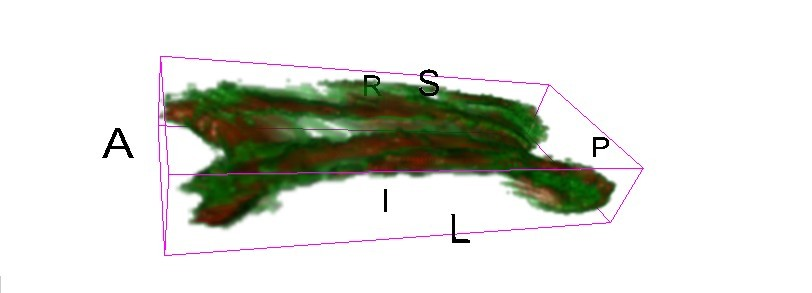
\includegraphics{pics/corpusA5.jpg}}
\end{minipage}
\begin{minipage}[b]{.45\linewidth}
\hspace{-0.2cm}
\centering
\scalebox{0.35}[0.26]{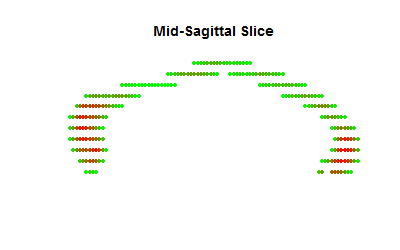
\includegraphics{pics/corpusA3.png}}
\end{minipage}
\end{figure}
176 patients with MS(Multiple Sclerosis), 466 scans.\

Color indicates corresponding FA.
\end{frame}

\begin{frame}
\frametitle{Pipeline}
\begin{enumerate}
\item Obtain the center curve (principal curve) of the target data cloud.
\item Measure the thickness.
\item Regress the thickness function on a scalar outcome.
\item Hypothesis testing.

%Awesome 
\end{enumerate}
\end{frame}

\begin{frame}
\frametitle{Simulation Settings}

For ease of computation, we first generate $Y_i$, ($i=1,2,...I$) and then generate $I$ shapes with features of the $i^{th}$ shape determined by the value of $Y_i$.

\bi
\item Case 1: I=300, response $Y_i\sim \text{Possion}(\lambda=3)$. Thickness of image$_i$ within $(\frac{\pi}{3},\frac{3\pi}{4})$ and $(\frac{5\pi}{4},\frac{7\pi}{4})$ is related to $Y_i$.
\begin{figure}[!th]
\centering
\scalebox{0.2}{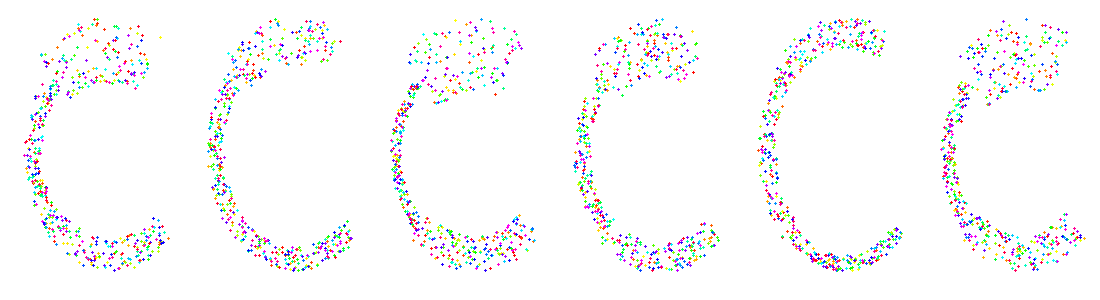
\includegraphics{pics/Simulation_C.png}}
\end{figure}\

\item Case 2: I=300, response $Y_i\sim \text{Possion}(\lambda=3)$. Thickness of image$_i$ in the vertical bar is related to $Y_i$.
\begin{figure}[!th]
\centering
\scalebox{0.2}{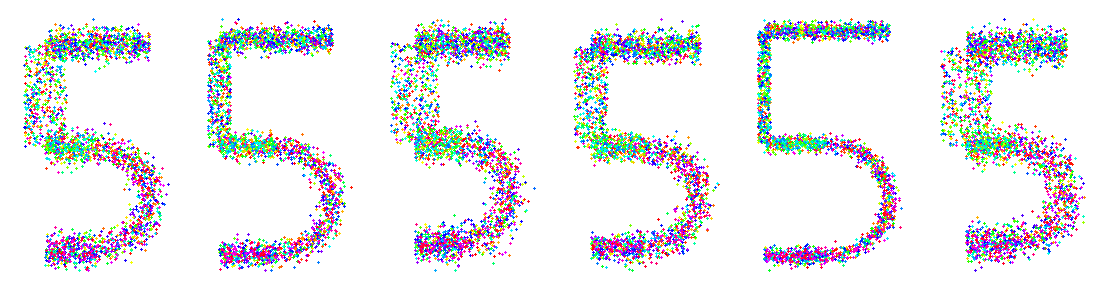
\includegraphics{pics/Simulation_5.png}}
\end{figure}
\ei
%The gray background goes really well with these colorful pictures!
\end{frame}

\section*{Curve Fitting}
\begin{frame}
\frametitle{Principal curve}
\begin{figure}[!th]
\centering
\begin{minipage}[b]{.45\linewidth}
\centering
\scalebox{0.3}{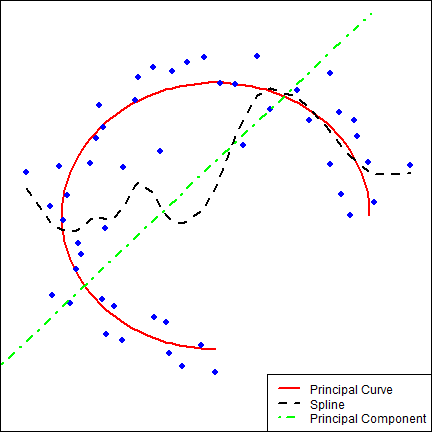
\includegraphics{pics/plot3.png}}
\end{minipage}
\begin{minipage}[b]{.45\linewidth}
\hspace{-.4cm}
\centering
\scalebox{0.25}[0.32]{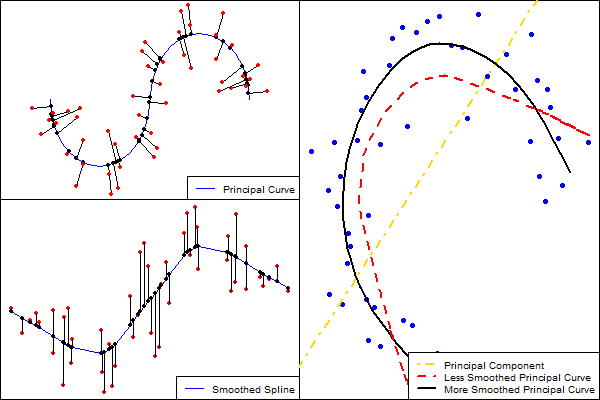
\includegraphics{pics/plot4.png}}
\end{minipage}
\end{figure}
\end{frame}

\begin{frame}
{\bf Principal Curve Algorithm}
\begin{enumerate}
\item{\bf The Projection Step.} The points are projected onto the curve of the previous iteration.
\item{\bf The Conditional Expectation Step.} For each data point $\xii$, we calculate a locally average $\bar{\mathbf{x}}^{(i)}$.
\item{\bf The Smoothing Step.} Fitting a fast TPS using all the local average data point $\bar{\mathbf{x}}^{(i)}$, obtain $f^{new}$.
\end{enumerate}
\begin{figure}[ht]
\begin{minipage}[b]{0.45\linewidth}
\centering
\scalebox{0.4}{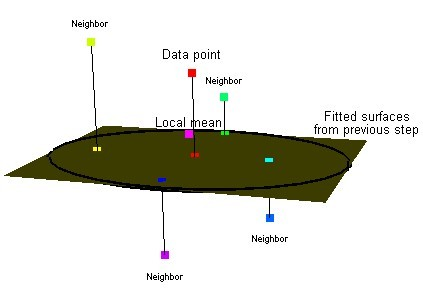
\includegraphics{pics/alg_1.jpg}}
\end{minipage}
\begin{minipage}[b]{0.45\linewidth}
\centering
\scalebox{0.4}{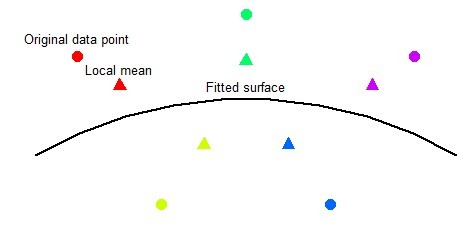
\includegraphics{pics/alg_2.jpg}}
\end{minipage}
\end{figure}
\end{frame}

\begin{frame}
\frametitle{Principal curve fitting result}
\begin{figure}[ht]
\centering
\scalebox{0.27}{\includegraphics{pics/Pcurve_C.png}}
\scalebox{0.27}{\includegraphics{pics/Pcurve_5.png}}
\end{figure}
\end{frame}

\begin{frame}
\frametitle{Obtaining Thickness along the principal curve}
\begin{itemize}
\item $\text{Thick}^*(t)=\text{Quantile}\big(\{2\times \text{dist}_{t_{j}},\big||t_{j}-t|\le.02\}\ 0.95\big)$
\item Fit a smooth spline of all $\text{Spline}(\text{Thick}^*(.)\longrightarrow\ \text{Thick}(.))$
\end{itemize}
\begin{figure}[ht]
\begin{minipage}[b]{0.45\linewidth}
\centering
\scalebox{0.27}{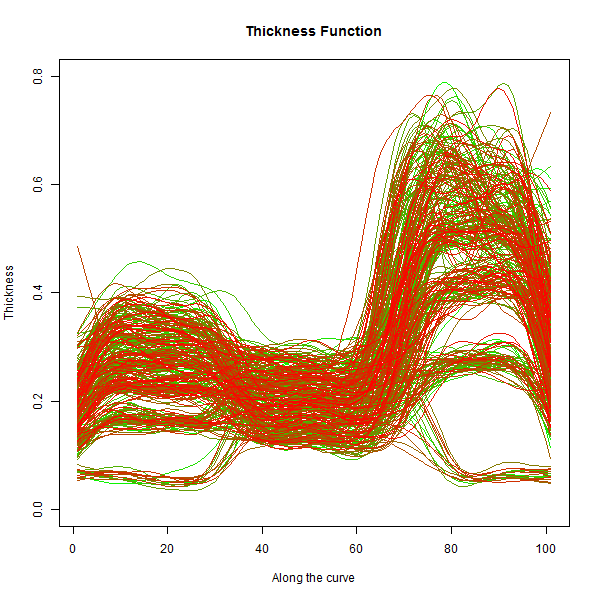
\includegraphics{pics/thickness.png}}
\end{minipage}
\begin{minipage}[b]{0.45\linewidth}
\centering
\scalebox{0.27}{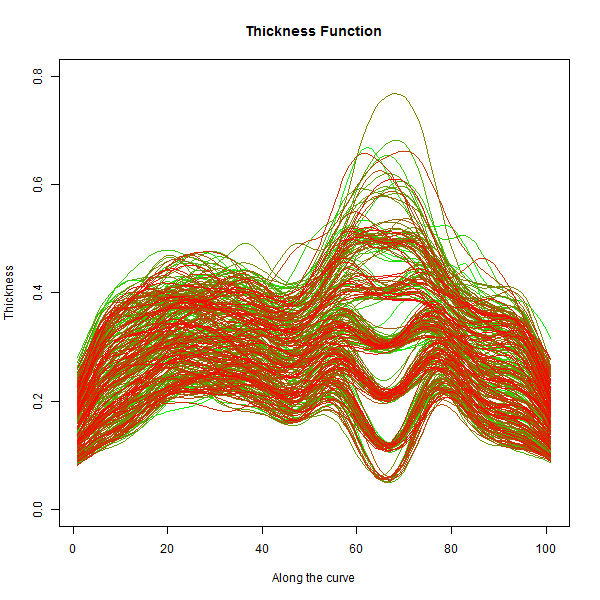
\includegraphics{pics/thickness2.png}}
\end{minipage}
\end{figure}
\end{frame}


\section*{Regression}
%%%%%%%%%%%%%%%%%%%%%%%%%%%%%%%%%%%%%%%%%%%%%%%%%
%%%%%%%%%%%%%%%%%%%%%%%%%%%%%%%%%%%%%%%%%%%%%%%%%
\begin{frame}{Regression Notation}

$Y_i$ = Outcome (simulated EDSS score) \\
$X_i(t)$= The thickness function along the track of the structure \\
$\beta(t)$ = Function representing effect of thickness on outcome, at different points.\\
$t \in [0,1]$.\\

\es{
Y_i \sim Poisson(\theta_i)\\
\theta_i =\beta_0 + \int_0^1 X_i(t)\beta(t) dt \\
}

\end{frame}
%%%%%%%%%%%%%%%%%%%%%%%%%%%%%%%%%%%%%%%%%%%%%%%%%
%%%%%%%%%%%%%%%%%%%%%%%%%%%%%%%%%%%%%%%%%%%%%%%%%



%%%%%%%%%%%%%%%%%%%%%%%%%%%%%%%%%%%%%%%%%%%%%%%%%
%%%%%%%%%%%%%%%%%%%%%%%%%%%%%%%%%%%%%%%%%%%%%%%%%
\begin{frame}{Regression Notation}

Estimate the functions $X_i(t)$ and $\beta(t)$ using basis functions.\

For $X$, we'll use it's principle components. For $\beta$, we'll use a b-spline basis.
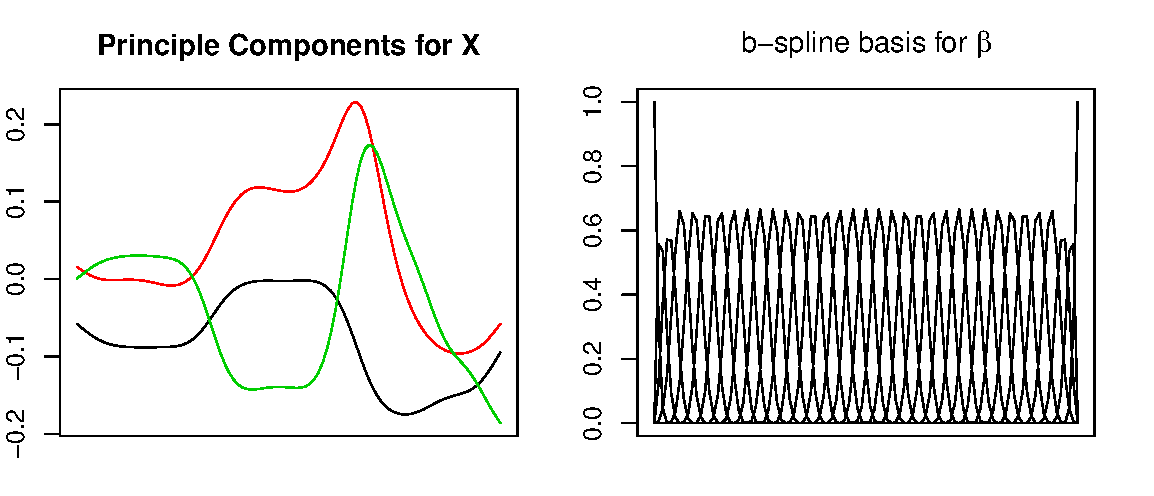
\includegraphics[scale=.5]{pics/Figure_Basis.pdf}
\es{
X_i(t) \approx \sum_{k=1}^{K_x} \xi_{ik} \Psi_k(t) \hspace{2.3cm} \beta(t) \approx \sum_{l=1}^{K_\beta} \beta_l \varphi_l(t) 
}
\end{frame}
%%%%%%%%%%%%%%%%%%%%%%%%%%%%%%%%%%%%%%%%%%%%%%%%%
%%%%%%%%%%%%%%%%%%%%%%%%%%%%%%%%%%%%%%%%%%%%%%%%%


%%%%%%%%%%%%%%%%%%%%%%%%%%%%%%%%%%%%%%%%%%%%%%%%%
%%%%%%%%%%%%%%%%%%%%%%%%%%%%%%%%%%%%%%%%%%%%%%%%%
\begin{frame}{Regression Notation}

\es{
\int_0^1 X_i(t)\beta(t) dt & \approx \int_0^1 \left( \sum_{k\in \{A\} } \xi_{ik} \Psi_k(t) \right) \left( \sum_{ j\in \{ B\}} \beta_l \varphi_l(t)  \right)dt   \\
 &=\int_0^1 \left(  \sum_{(k,j)\in \{A\}\times \{B\} } \xi_{ik} \Psi_k(t)    \varphi_l(t)   \beta_l \right) dt \\
 &=  \sum_{(k,j)\in \{A\}\times \{B\} } \xi_{ik}  \left( \int_0^1 \Psi_k(t)    \varphi_l(t)  dt \right) \beta_l  \\
 &=: \xi_{i} \bold{J} \beta^T  \\
 }
 
 \bi
\item  Where $\xi_i=[\xi_{i1},..\xi_{iK_X}]^T$, $\beta=[\beta_1,...\beta_{K_\beta}]^T$, and $\bold{J}$ is a $K_x \times K_\beta$ matrix with $(i,j)^{th}$ element equal to $ \int_0^1 \Psi_i(t)    \varphi_j(t) dt$. 
\item For this project we'll assume $\xi_{i} \bold{J}$ is fixed, and will put a penalty prior on $\beta$.
\ei

%%%%%% DO WE NEED A BETA 0 IF OUR FIRST PC IS FLAT????? (it's not...)

\end{frame}
%%%%%%%%%%%%%%%%%%%%%%%%%%%%%%%%%%%%%%%%%%%%%%%%%
%%%%%%%%%%%%%%%%%%%%%%%%%%%%%%%%%%%%%%%%%%%%%%%%%


%%%%%%%%%%%%%%%%%%%%%%%%%%%%%%%%%%%%%%%%%%%%%%%%%
%%%%%%%%%%%%%%%%%%%%%%%%%%%%%%%%%%%%%%%%%%%%%%%%%
\begin{frame}{Full Model}

\es{
Y_i \sim Poisson(\theta_i) \\
 \theta_i  = \beta_0+ \xi_{i} \bold{J} \beta^T  \\
\beta_0, \beta_1 \sim N(0,100) \\
 \beta_j \sim N(\beta_{j-1},1/\tau_\beta) \\
 \tau_\beta \sim \Gamma(.001,.001)\\
 }

This could be made to account for measurement error by letting: $W_i(t)=
\sum_{k=1}^{K_x} \xi_{ik} \Psi_k(t) + \epsilon_i(t)$, and assigning priors for $\epsilon_i(t)$ and $\xi_{ik}$.\vspace{.1cm}


 
 Fit this in WinBUGS. \footnote{(Crainiceanu and Goldsmith 2010; Brezger, Kneib, and Lang 2005; Lang and Brezger 2004; Goldsmith, Feder, Crainiceanu, Caffo, and Reich, 2010)}


\end{frame}
%%%%%%%%%%%%%%%%%%%%%%%%%%%%%%%%%%%%%%%%%%%%%%%%%
%%%%%%%%%%%%%%%%%%%%%%%%%%%%%%%%%%%%%%%%%%%%%%%%%



\section*{Testing}
%%%%%%%%%%%%%%%%%%%%%%%%%%%%%%%%%%%%%%%%%%%%%%%%%
%%%%%%%%%%%%%%%%%%%%%%%%%%%%%%%%%%%%%%%%%%%%%%%%%
\begin{frame}{Hypothesis Testing}

%%%%%%%% !!!!!! ????? Add mini figure!!!

Given draws ($\beta_d(t)$) from the posterior:
\bi
\item Credible intervals give the range along the curve where 95\% of the points will fall
\ilist{To estimate this, we need the quantiles for $\beta_d(t)$.}
\item Credible bands give the area within which 95\% of the curves will be completely contained
\ilist{Roughly speaking, we'd need the quantiles for each curve's largest deviation from the mean curve.}
\ei 

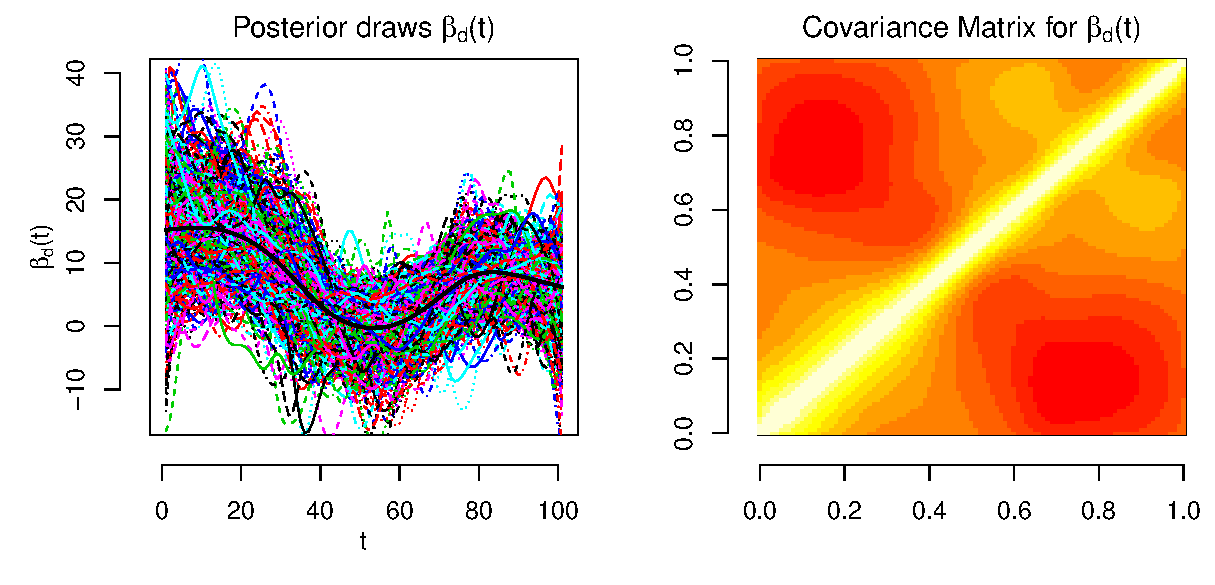
\includegraphics[scale=.5]{pics/Figure_BtDraws_&_Cov_C_35.pdf}

\end{frame}
%%%%%%%%%%%%%%%%%%%%%%%%%%%%%%%%%%%%%%%%%%%%%%%%%
%%%%%%%%%%%%%%%%%%%%%%%%%%%%%%%%%%%%%%%%%%%%%%%%%


%%%%%%%%%%%%%%%%%%%%%%%%%%%%%%%%%%%%%%%%%%%%%%%%%
%%%%%%%%%%%%%%%%%%%%%%%%%%%%%%%%%%%%%%%%%%%%%%%%%
\begin{frame}{Hypothesis Testing}

\begin{columns}[c]
 \column{.5\textwidth}

Let:
\bi
\item $\hat{\beta}(t)=mean(\beta_d(t))$
\item $\sigma(t)^2 = var(\beta_d(t))$
\item $S_d(t) = \frac{|\beta_d(t)-\hat{\beta}(t)    | } {\sigma(t)}$
\ilist{Assume $P(S_d(t)>s)$ is constant over $t$, given $s$}
\item $m_d= max_t \left\lbrace S_d(t) \right\rbrace$
\item $q(m_d,.95)$ is the 95\% quantile of $m_d$ across $d$.
\item Reconstruct credible bands using $\hat{\beta}(t) \pm  q(m_d,.95)\sigma(t)$.
\ei


\column{.5\textwidth}
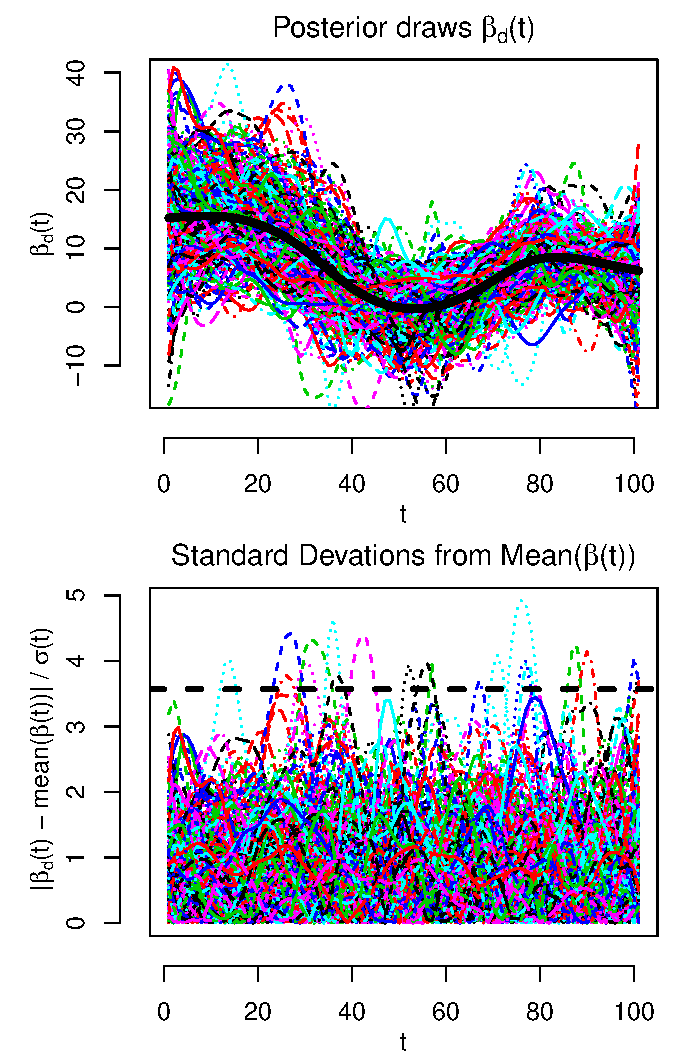
\includegraphics[scale=.4]{pics/Figure_Get_d_dist.pdf}
\end{columns} 

\end{frame}
%%%%%%%%%%%%%%%%%%%%%%%%%%%%%%%%%%%%%%%%%%%%%%%%%
%%%%%%%%%%%%%%%%%%%%%%%%%%%%%%%%%%%%%%%%%%%%%%%%%

%%%%%%%%%%%%%%%%%%%%%%%%%%%%%%%%%%%%%%%%%%%%%%%%%
%%%%%%%%%%%%%%%%%%%%%%%%%%%%%%%%%%%%%%%%%%%%%%%%%
\begin{frame}{Credible Intervals \& Bands - C Shape}

\begin{center}

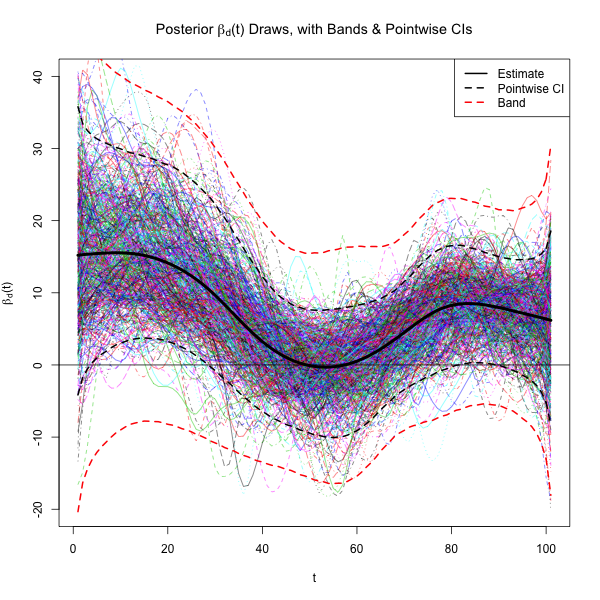
\includegraphics[scale=.37]{pics/Figure_Bands_C_Shape_12-19-12_Nobonf.png}

\end{center}
\end{frame}
%%%%%%%%%%%%%%%%%%%%%%%%%%%%%%%%%%%%%%%%%%%%%%%%%
%%%%%%%%%%%%%%%%%%%%%%%%%%%%%%%%%%%%%%%%%%%%%%%%%



%%%%%%%%%%%%%%%%%%%%%%%%%%%%%%%%%%%%%%%%%%%%%%%%%
%%%%%%%%%%%%%%%%%%%%%%%%%%%%%%%%%%%%%%%%%%%%%%%%%
\begin{frame}{Comparison to a Bonferroni}

\bi
\item Pointwise intervals above are calculated above using the (.5$\alpha$) \& (1-$.5/alpha$) quantiles at each point $t$ (with $\alpha= .05$).
\item We could also create a confidence band using a Bonferroni style adjustment, using the ($.5\alpha/100$) and $(1- \frac{.5\alpha}{ 100})$
%% Add more explanation???? !!!!!!!!!!  \ilist{}
\ei



\end{frame}
%%%%%%%%%%%%%%%%%%%%%%%%%%%%%%%%%%%%%%%%%%%%%%%%%
%%%%%%%%%%%%%%%%%%%%%%%%%%%%%%%%%%%%%%%%%%%%%%%%%


%%%%%%%%%%%%%%%%%%%%%%%%%%%%%%%%%%%%%%%%%%%%%%%%%
%%%%%%%%%%%%%%%%%%%%%%%%%%%%%%%%%%%%%%%%%%%%%%%%%
\begin{frame}{Credible Intervals \& Bands - C Shape}

\begin{center}

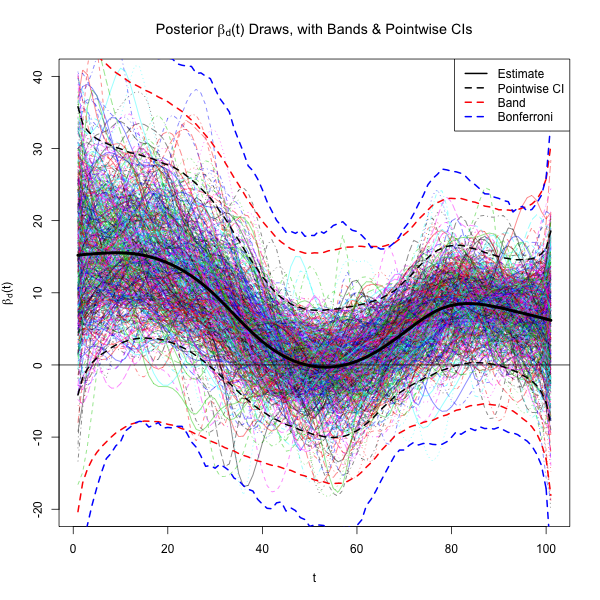
\includegraphics[scale=.37]{pics/Figure_Bands_C_Shape_12-19-12_bonf.png}

\end{center}
\end{frame}
%%%%%%%%%%%%%%%%%%%%%%%%%%%%%%%%%%%%%%%%%%%%%%%%%
%%%%%%%%%%%%%%%%%%%%%%%%%%%%%%%%%%%%%%%%%%%%%%%%%


%%%%%%%%%%%%%%%%%%%%%%%%%%%%%%%%%%%%%%%%%%%%%%%%%
%%%%%%%%%%%%%%%%%%%%%%%%%%%%%%%%%%%%%%%%%%%%%%%%%
\begin{frame}{Credible Intervals \& Bands - 5 Shape}

\begin{center}

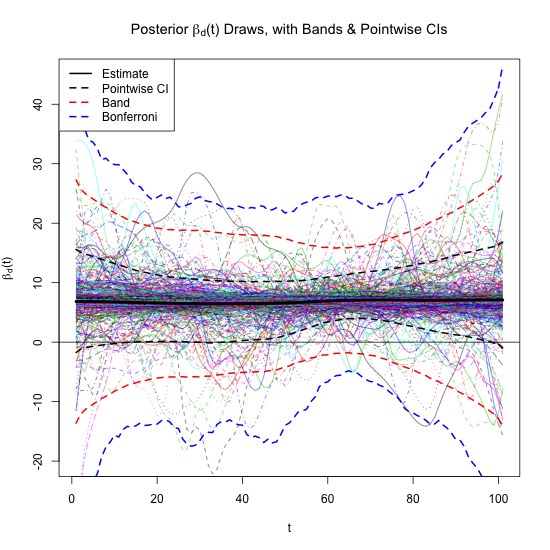
\includegraphics[scale=.37]{pics/Figure_Bands_5_Shape_12-19-12_bonf.png}

\end{center}
\end{frame}
%%%%%%%%%%%%%%%%%%%%%%%%%%%%%%%%%%%%%%%%%%%%%%%%%
%%%%%%%%%%%%%%%%%%%%%%%%%%%%%%%%%%%%%%%%%%%%%%%%%


%%%%%%%%%%%%%%%%%%%%%%%%%%%%%%%%%%%%%%%%%%%%%%%%%
%%%%%%%%%%%%%%%%%%%%%%%%%%%%%%%%%%%%%%%%%%%%%%%%%
\begin{frame}{Discussion}
\bi
\item The credible band never rises above zero, but several points are pointwise significant. These could be the subject of future tests if they were real data. \vspace{.4cm}
\item Principle curve procedure sometimes doesn't work so well at the end points, it they are too thick.
\item Results are slightly sensitive to number of splines chosen.
\ei
\end{frame}
\end{document} 
%%%%%%%%%%%%%%%%%%%%%%%%%%%%%%%%%%%%%%%%%%%%%%%%%
%%%%%%%%%%%%%%%%%%%%%%%%%%%%%%%%%%%%%%%%%%%%%%%%%
